% coding: utf-8


% \documentclass[a4paper, 10pt]{jarticle}
\documentclass[a4paper, report, 10.5pt]{jsbook}


\usepackage{bm}
\usepackage{comment}
\usepackage{amssymb}
\usepackage{amsmath}
\usepackage[dvipdfmx]{graphicx}
\usepackage{listings,jvlisting} %日本語のコメントアウトをする場合jlisting(もしくはjvlisting)が必要
%ここからソースコードの表示に関する設定
\lstset{
  basicstyle={\ttfamily},
  identifierstyle={\small},
  commentstyle={\smallitshape},
  keywordstyle={\small\bfseries},
  ndkeywordstyle={\small},
  stringstyle={\small\ttfamily},
  frame={tb},
  breaklines=true,
  columns=[l]{fullflexible},
  numbers=left,
  xrightmargin=0zw,
  xleftmargin=3zw,
  numberstyle={\scriptsize},
  stepnumber=1,
  numbersep=1zw,
  lineskip=-0.5ex
}
%ここまでソースコードの表示に関する設定
\usepackage{hyperref}
\def\figureautorefname~#1\null{ 図~#1\null}
\def\tableautorefname~#1\null{ 表~#1\null}
\def\sectionautorefname~#1\null{第~#1章\null}
\def\subsectionautorefname~#1\null{~#1節\null}
\def\subsubsectionautorefname~#1\null{~#1節\null}
\newif\iffigure
% \figurefalse
\figuretrue


\title{画像処理技術における信号処理技術の応用 \\
      \Large{確率解析信号特論 課題レポート}}
\author{創成科学研究科 基盤科学系専攻 情報コース \\
        20-8801-037-4 \\
        寄元康平}
\date{}


\begin{document}
\maketitle
\chapter{はじめに}


信号処理技術とは,信号データの計測や解析,また解析するための技術を指す.
具体的には,音声や回路の電流値といったような計測器から計測されたアナログデータを
デジタルデータへサンプリング処理,
データに含まれている周波数成分の解析やデータの特徴となる周波数領域の抽出,
また計測時に生じたノイズを除去するためのフィルタ処理が挙げられ,
デジタルデータの前処理や音声の合成などに応用されている.
一方で,画像処理技術とは,画像における情報の解析,抽出や必要に応じた加工などのような画像データに対して
行われる処理技術の総称である.
具体的な例としては画像内のノイズ除去,輪郭の抽出,拡大や縮小,パターンマッチングなどが挙げられる.
これらの技術はレントゲン写真,CTスキャンの取得や解析といった医療現場,工場での製品の異常検知,
また撮影した画像に対しての編集といったような我々の身の回りの画像に対して幅広く活用されている.
最近では,コンピュータの発展に伴い機械学習技術を導入したより高度でかつ高精度な
画像処理技術が研究,開発されている.
信号処理技術には,データ内のノイズ除去や必要となる特徴の抽出などのように画像処理技術と
共通する技術がいくつか存在する.
このことから信号処理技術に用いられているフィルタ処理を画像処理に活用できるではないかと
考えた.

本レポートでは,信号処理技術における一部のフィルタ処理を画像データに対して活用する
実験,検証を行った.

\chapter{信号処理技術}


本章では時間領域の離散データを周波数領域の離散データに変換する離散フーリエ変換,
また時間領域のデータから特定の周波数領域を抽出するフィルタ処理であるバンドパスフィルタに
ついて紹介する.


% \input{documents/a_fourier}
\section{離散フーリエ変換}

音声や電流といった信号を計測したとき,それらの値は時間領域における電気信号の連続データ(アナログデータ)
として出力される.
連続データはコンピュータ上で扱うことができないので,連続データを
ある一定間隔でサンプリングすることでコンピュータ上で扱える離散データ(デジタルデータ)
へ変換することでコンピュータ上でのデータの取得,解析が可能となる(\autoref{fig:digital_sin}).
\iffigure
\begin{figure}[h]
  \centering
  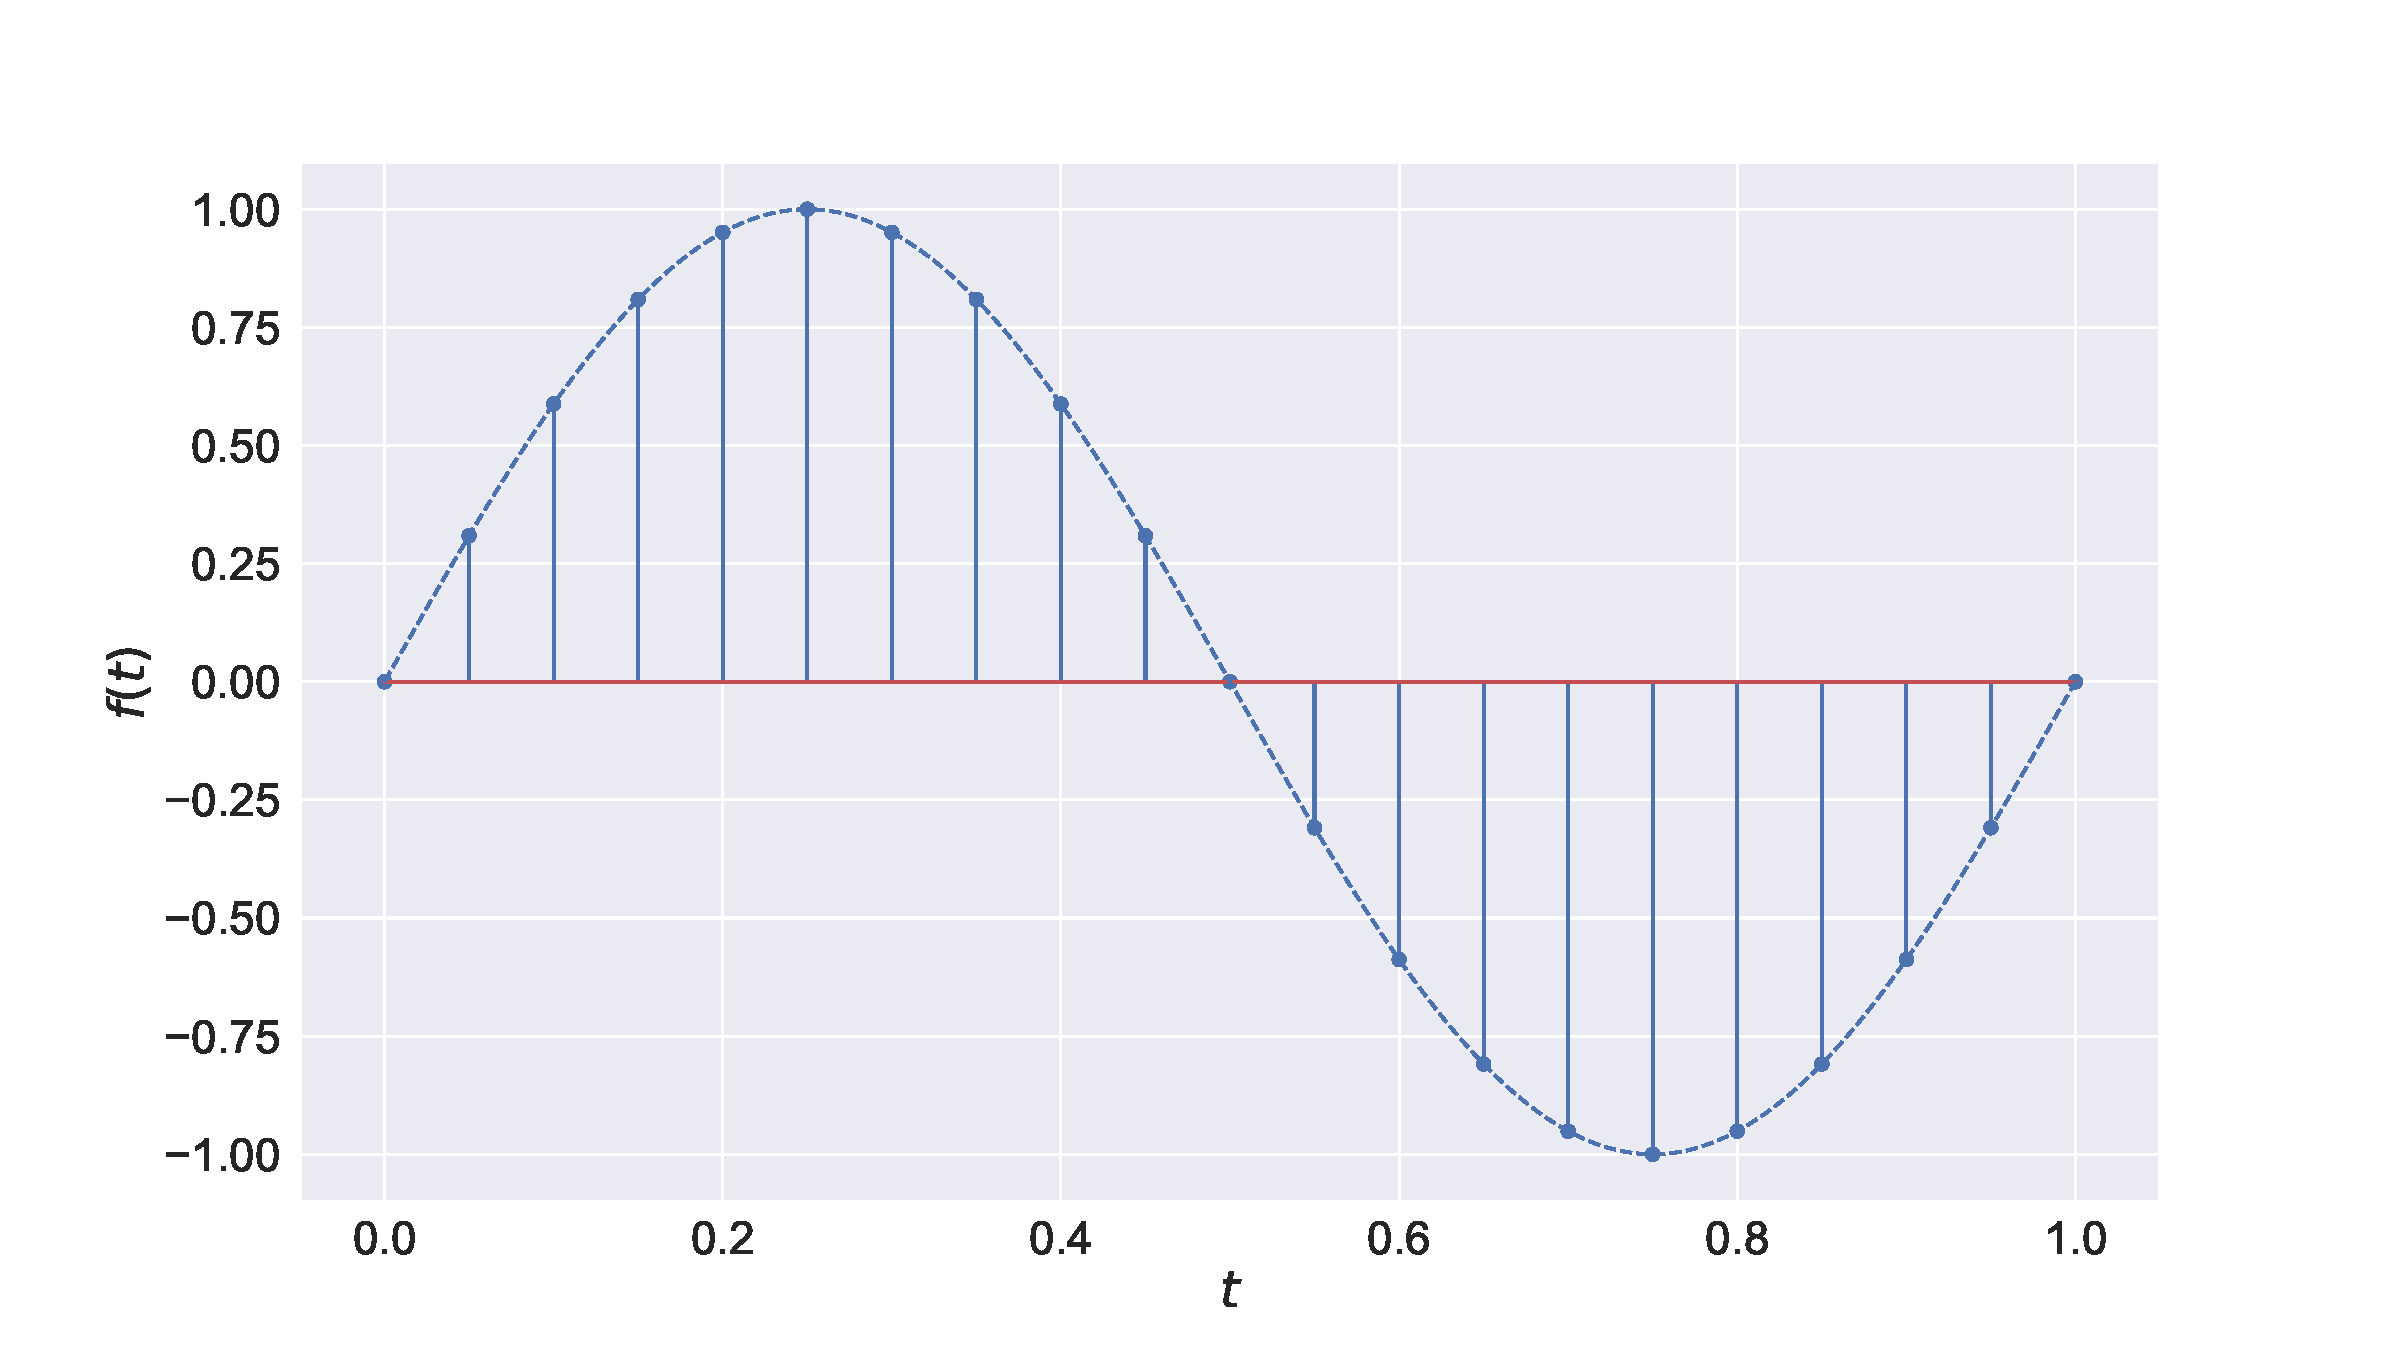
\includegraphics[clip, width=\textwidth]{figure/sin.pdf}
  \caption{離散データの一例}
  \label{fig:digital_sin}
\end{figure}
\fi

この離散データに含まれている周波数成分を算出する手法として離散フーリエ変換が存在する.
離散フーリエ変換とは,式(\ref{eq:dft})で定義される手法であり,
時間領域の離散データ$f(t)$を周波数領域の離散データ$F(\omega)$へ変換することができる.
\begin{align}
  F(\omega) = \sum_{t=0}^{N-1} f(t) e ^ {-j \frac{2 \pi \omega}{N} t} \label{eq:dft}
\end{align}
このとき,式(\ref{eq:dft})における$N$は$f(t)$におけるデータ数である.
式(\ref{eq:dft})では,時間領域の実空間データを複素数空間における三角関数の
総和の形へ変換することにより,時間領域のデータに含まれている周波数成分を算出できる(\autoref{fig:dft}).
\autoref{fig:dft}は\autoref{fig:digital_sin}を離散フーリエ変換したときの周波数領域
データを示している.これより,\autoref{fig:digital_sin}のデータは,1Hz, 6Hz, 10Hzの周波数を
含むことがわかる.

また,周波数領域$F(\omega)$は離散フーリエ逆変換(式(\ref{eq:idft}))
を用いることで時間領域の離散データ$f(t)$へ復元することができる(\autoref{fig:idft}).
\begin{align}
  f(t) = \frac{1}{N}\sum_{\omega=0}^{N-1} F(\omega) e ^ {j \frac{2 \pi t}{N} \omega} \label{eq:idft}
\end{align}
\iffigure
\begin{figure}[h]
  \begin{minipage}{.45\hsize}
    \centering
    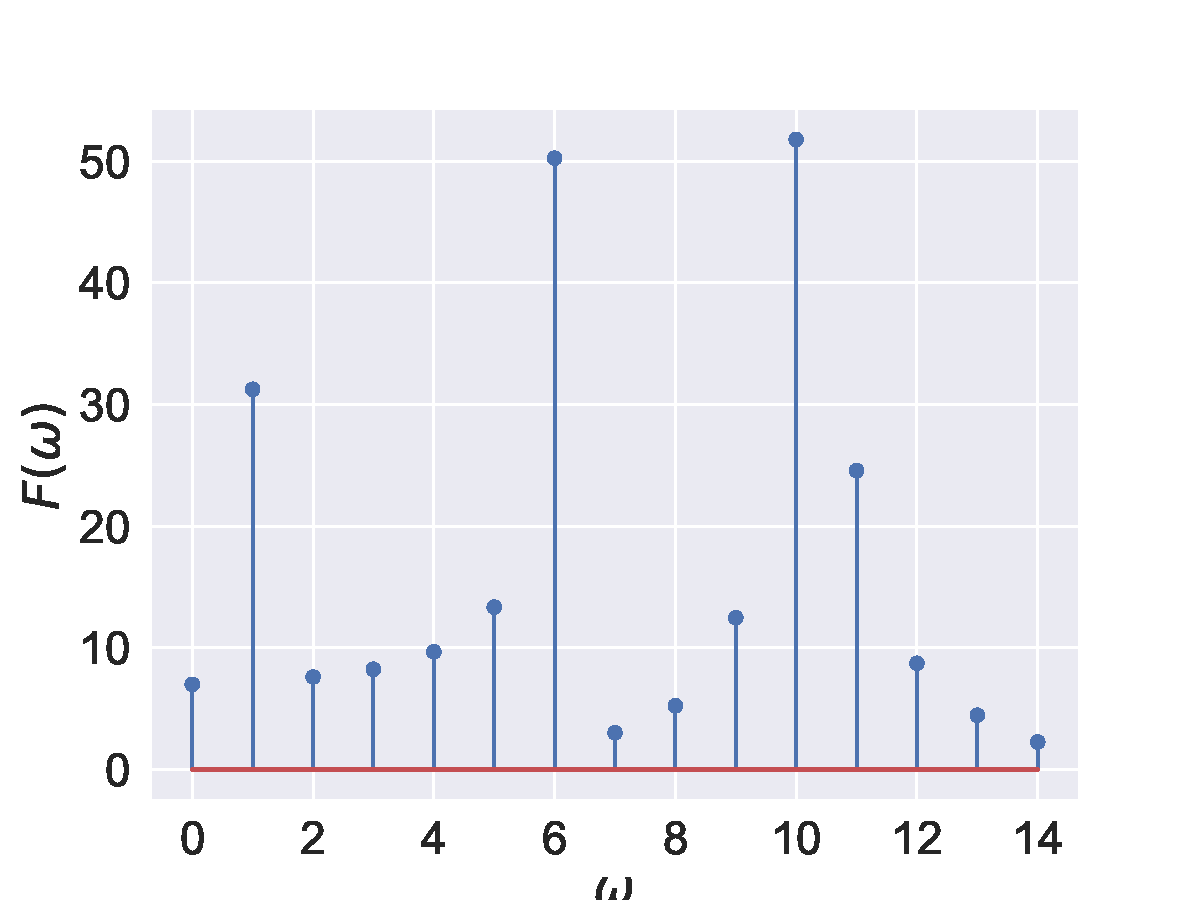
\includegraphics[clip, width=\textwidth]{figure/sin_dft.pdf}
    \caption{\autoref{fig:digital_sin}を式(\ref{eq:dft})を用いて周波数領域の離散データに変換}
    \label{fig:dft}
  \end{minipage}
  \begin{minipage}{.45\hsize}
    \centering
    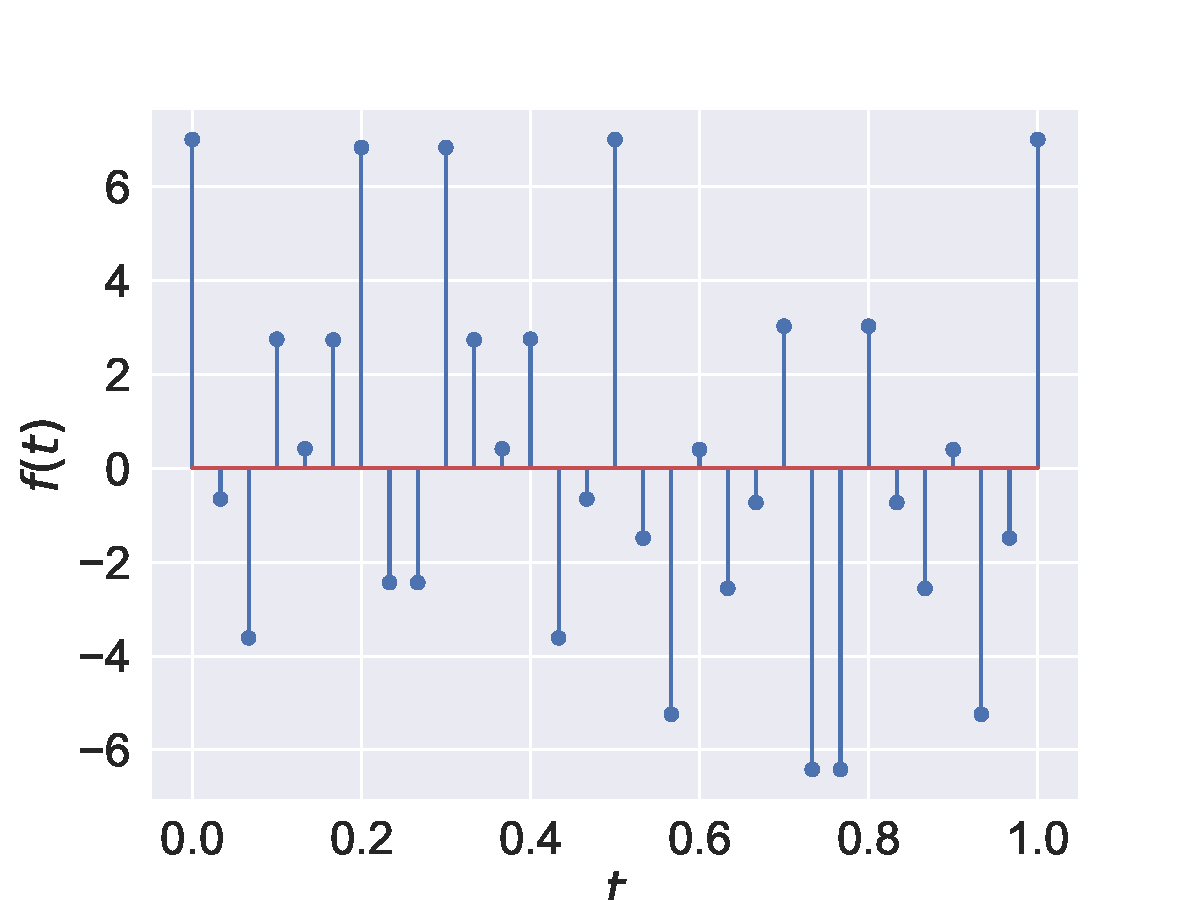
\includegraphics[clip, width=\textwidth]{figure/sin_idft.pdf}
    \caption{\autoref{fig:dft}を式(\ref{eq:idft})を用いて時間領域の離散データに逆変換}
    \label{fig:idft}
  \end{minipage}
\end{figure}
\fi

\section{バンドパスフィルタ}


離散フーリエ変換によって算出された周波数領域のデータにおいて,ある範囲の
周波数成分のみを抽出し時間領域のデータに逆変換するフィルタ処理のことを
バンドパスフィルタという.
このとき,抽出する周波数成分の閾値のことをカットオフ周波数という.
バンドパスフィルタは,計測したデータにノイズが含まれている場合や任意の周波数を含む
信号のみを計測する場合などに活用される.
\autoref{fig:band_pass}, \autoref{fig:band_ipass}にバンドパスフィルタを\autoref{fig:digital_sin}に対して行った例を示す.
\autoref{fig:band_pass}では,バンドパスフィルタを用いて$3 \le \omega \le 7$の周波数を抽出しており,
\autoref{fig:band_ipass}において6Hzのみのデータが抽出できていることがわかる.

\iffigure
\begin{figure}[h]
  \begin{minipage}{.45\hsize}
    \centering
    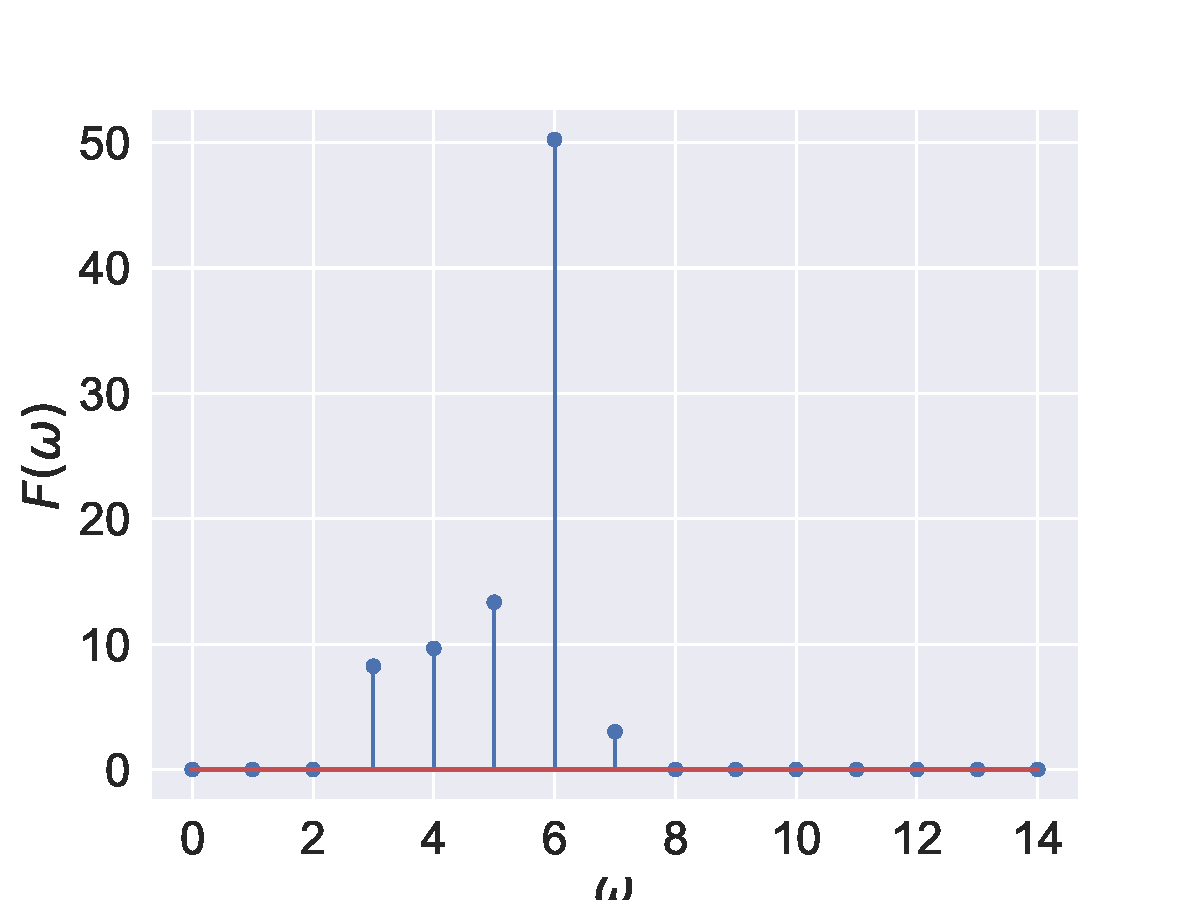
\includegraphics[clip, width=\textwidth]{figure/band_pass_dft.pdf}
    \caption{\autoref{fig:dft}に対してバンドパスフィルタを行った場合(周波数領域)}
    \label{fig:band_pass}
  \end{minipage}
  \begin{minipage}{.45\hsize}
    \centering
    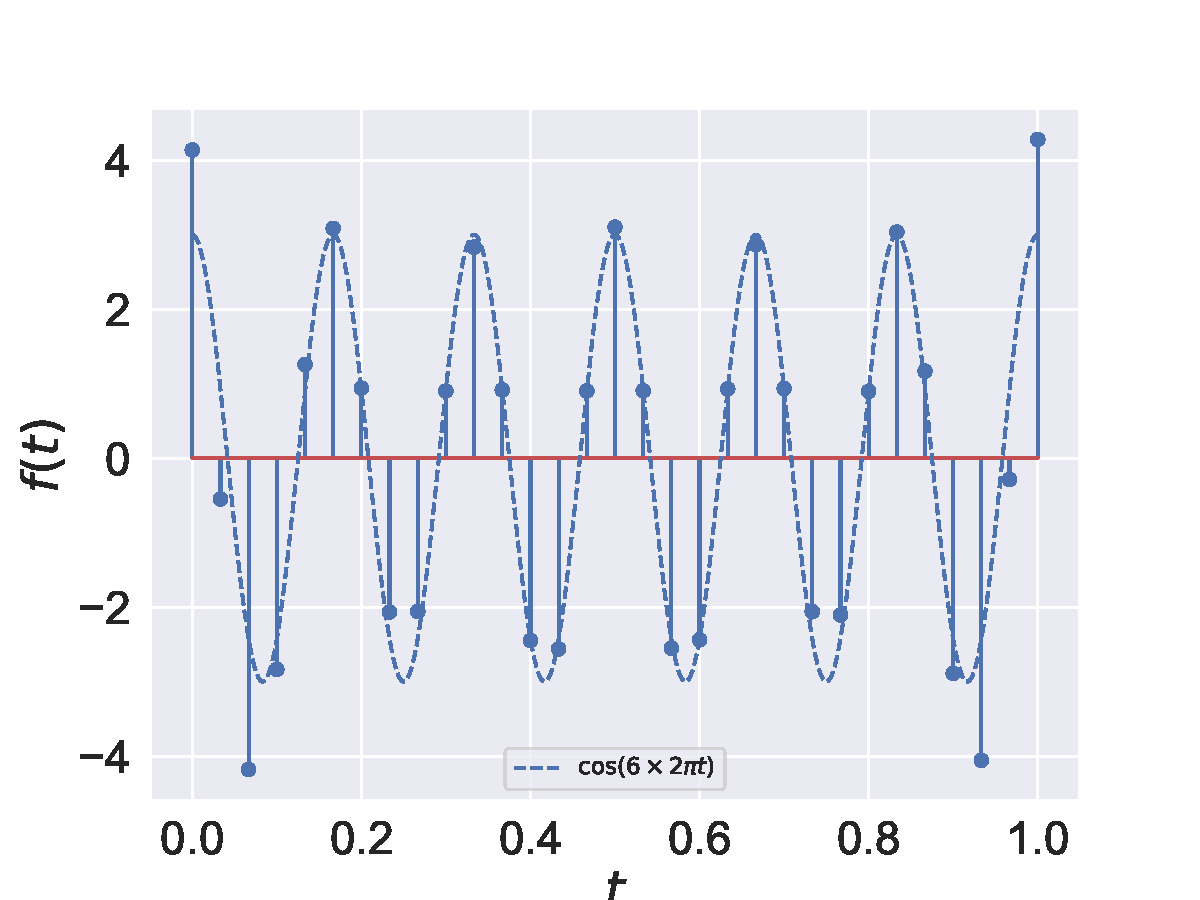
\includegraphics[clip, width=\textwidth]{figure/band_pass_idft.pdf}
    \caption{\autoref{fig:dft}に対してバンドパスフィルタを行った場合(時間領域)}
    \label{fig:band_ipass}
  \end{minipage}
\end{figure}
\fi
バンドパスフィルタにおいて,単一のカットオフ周波数以上の範囲のみを
抽出し高周波領域のデータを抽出するフィルタ処理をハイパスフィルタという.
\autoref{fig:band_pass}, \autoref{fig:band_ipass}にハイパスフィルタを\autoref{fig:digital_sin}に対して行った例を示す.
\autoref{fig:band_pass}では,ハイパスフィルタを用いて$7 \le \omega \le 14$の周波数を抽出しており,
\autoref{fig:band_ipass}において10Hzのみのデータが抽出できていることがわかる.

\iffigure
\begin{figure}[h]
  \begin{minipage}{.45\hsize}
    \centering
    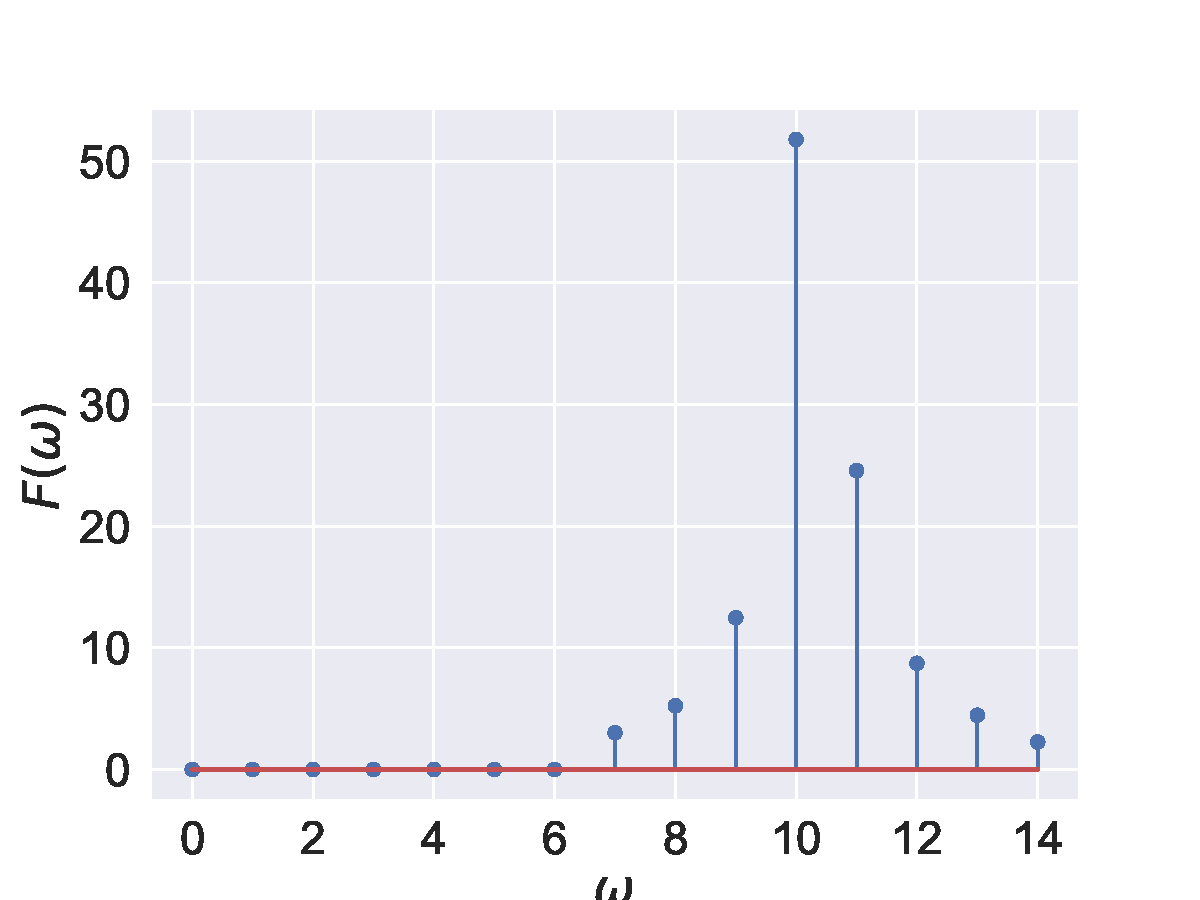
\includegraphics[clip, width=\textwidth]{figure/high_pass_dft.pdf}
    \caption{\autoref{fig:dft}に対してハイパスフィルタを行った場合(周波数領域)}
    \label{fig:high_sin}
  \end{minipage}
  \begin{minipage}{.45\hsize}
    \centering
    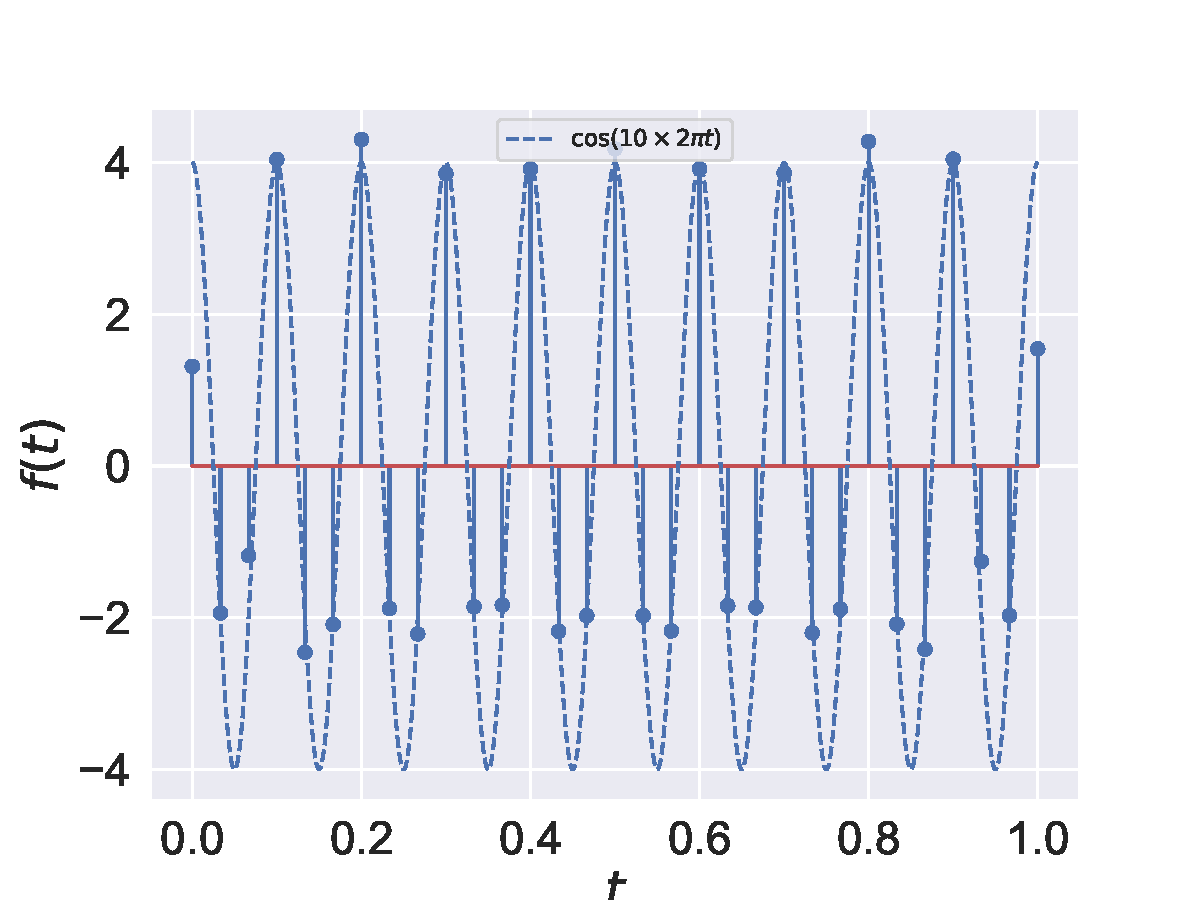
\includegraphics[clip, width=\textwidth]{figure/high_pass_idft.pdf}
    \caption{\autoref{fig:dft}に対してハイパスフィルタを行った場合(時間領域)}
    \label{fig:high_sin}
  \end{minipage}
\end{figure}
\fi

また,カットオフ周波数以下の範囲のみを
抽出し高周波領域のデータを抽出するフィルタ処理をローパスフィルタという.
\autoref{fig:low_pass}, \autoref{fig:low_ipass}にローパスフィルタを\autoref{fig:digital_sin}に対して行った例を示す.
\autoref{fig:low_pass}では,バンドパスフィルタを用いて$0 \le \omega \le 3$の周波数を抽出しており,
\autoref{fig:low_ipass}において1Hzのみのデータが抽出できていることがわかる.

\iffigure
\begin{figure}[h]
  \begin{minipage}{.45\hsize}
    \centering
    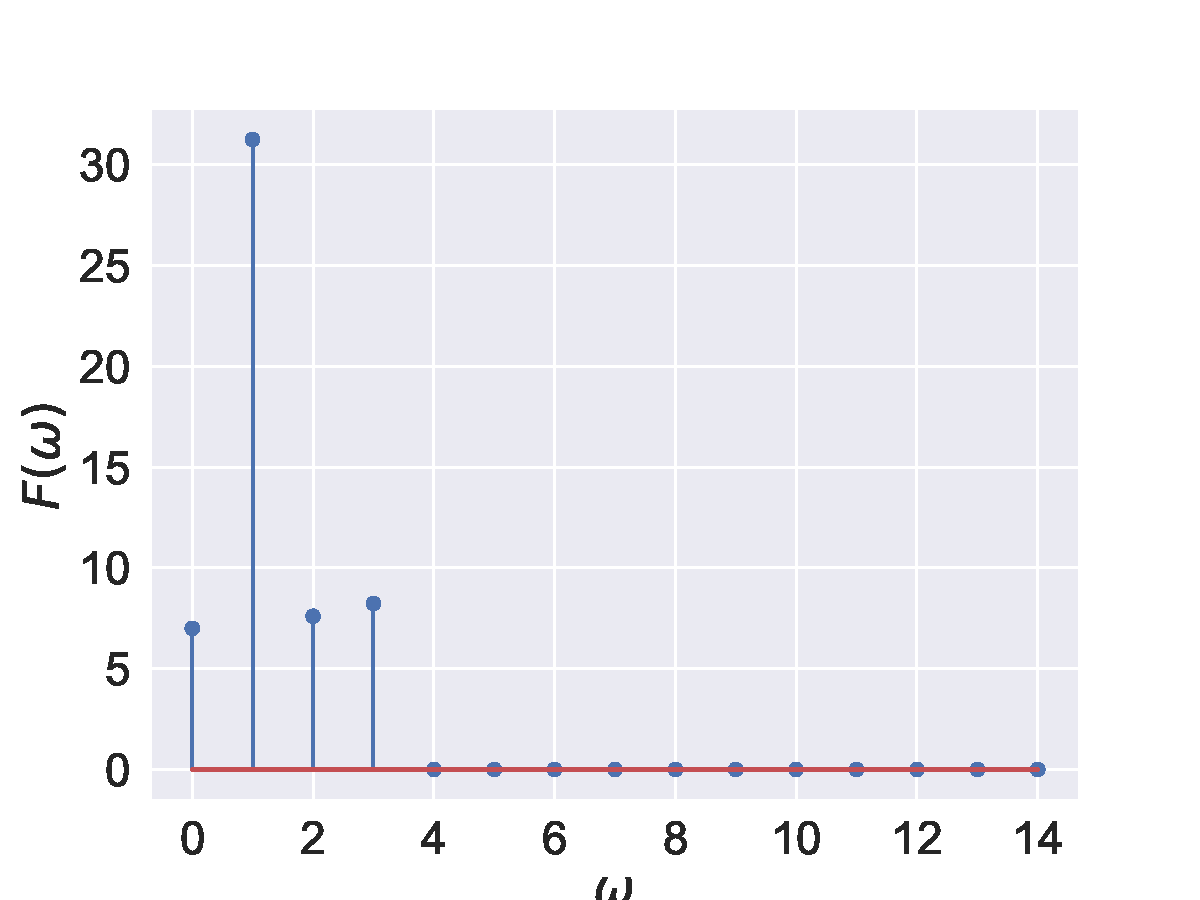
\includegraphics[clip, width=\textwidth]{figure/low_pass_dft.pdf}
    \caption{\autoref{fig:dft}に対してローパスフィルタを行った場合(周波数領域)}
    \label{fig:low_pass}
  \end{minipage}
  \begin{minipage}{.45\hsize}
    \centering
    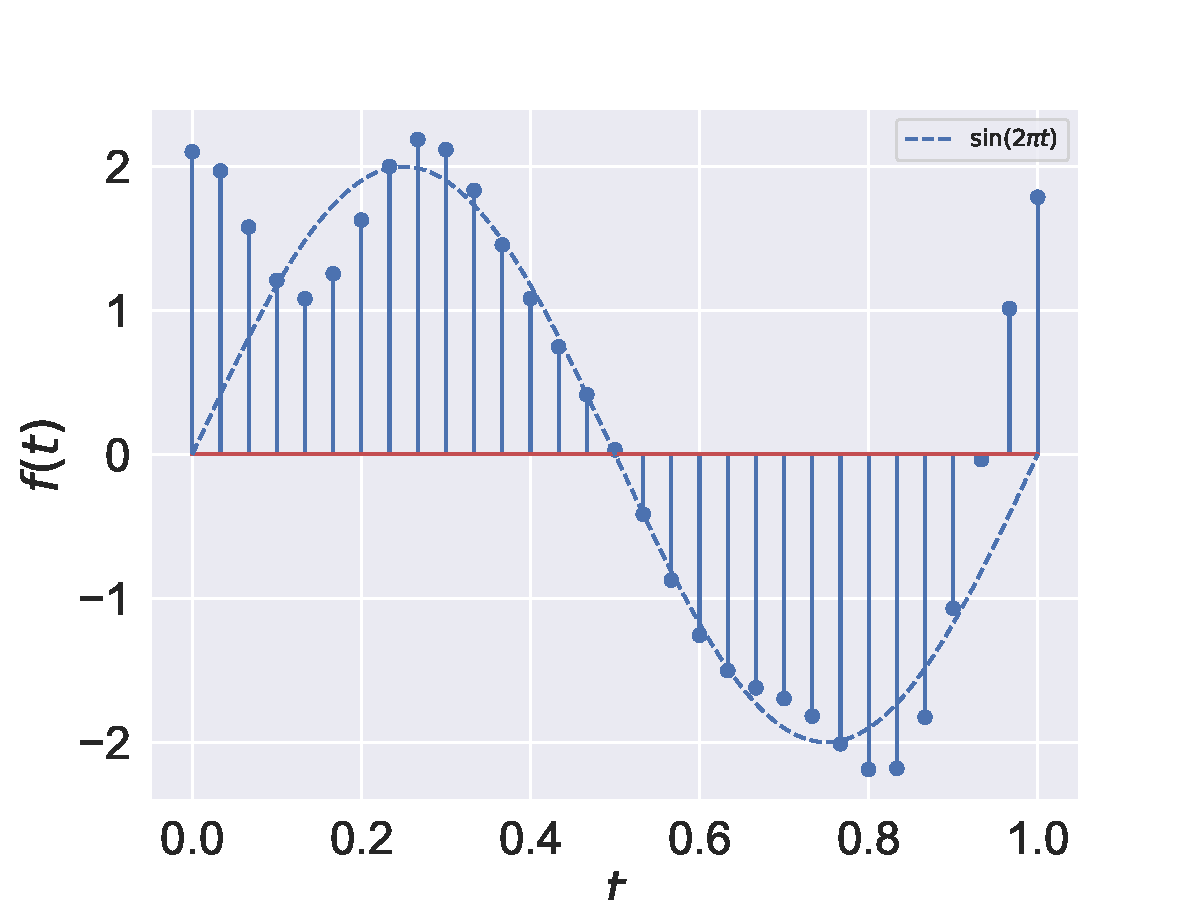
\includegraphics[clip, width=\textwidth]{figure/low_pass_idft.pdf}
    \caption{\autoref{fig:dft}に対してローパスフィルタを行った場合(時間領域)}
    \label{fig:low_ipass}
  \end{minipage}
\end{figure}
\fi

% \input{documents/low_path}
% \input{documents/high_path}

\chapter{信号処理技術の画像データへの応用}

本章では,離散フーリエ変換の画像データへの応用について紹介し,
また信号処理におけるフィルタ処理の一部を画像データへ活用する.
なお,実装する環境を以下に示す.


\begin{itemize}
  \item OS: Windows10
  \item プログラム言語: Python 3.6
  \item ライブラリ
  \begin{itemize}
    \item NumPy: 数値計算ライブラリ
    \item OpenCV: 画像処理ライブラリ
    \item MatPlotLib: 画像出力ライブラリ
  \end{itemize}
\end{itemize}

\section{離散フーリエ変換の画像データへの応用}

これまでの離散フーリエ変換(式(\ref{eq:dft}))は時間空間の1次元離散データにおける
周波数成分を抽出し,離散逆フーリエ変換(式(\ref{eq:idft}))を用いて
時間領域のデータへ復元していた.
この1次元データ上での離散フーリエ変換を画像データへ応用するには,画像を2次元の
時間空間における離散データ$f(x, y)$とみなし,$x, y$それぞれの方向に対して
離散フーリエ変換(式(\ref{eq:dft_2d}))することで,2次元の周波数成分$F(u, v)$を算出できる.
\begin{align}
  F(u, v) = \sum_{x = 0}^{M-1} \sum_{y = 0}^{N-1} f(x, y) e ^ {- 2 \pi \left(\frac{ux}{M} + \frac{vy}{N} \right) j} \label{eq:dft_2d}
\end{align}
\autoref{fig:input_example},\autoref{fig:dft_example}
に画像データへ離散フーリエ変換を行った例を示す.
\autoref{fig:input_example}は入力画像であり,
\autoref{fig:dft_example}は入力画像の周波数領域である.
この図では,図の中心に近い領域は低周波成分を示し,中心から離れていくほど高周波成分を示している.
\autoref{Fig:dft_example}に対して信号処理にて用いられているバンドパスフィルタを
用いることで信号処理技術でのフィルタ処理を画像データに応用できる.

離散フーリエ逆変換も式(\ref{eq:dft_2d})と同様に$(u, v)$それぞれの方向に対して
逆変換を行うことで\autoref{fig:dft_example}から元の画像へ復元できる(式(\ref{eq:idft_2d})).
\begin{align}
  f(x, y) = \frac{1}{MN} \sum_{u = 0}^{M-1} \sum_{v = 0}^{N-1} F(u, v) e ^ {2 \pi \left(\frac{ux}{M} + \frac{vy}{N} \right) j} \label{eq:idft_2d}
\end{align}
\iffigure
\begin{figure}[h]
  \centering
  \begin{minipage}{.45\hsize}
    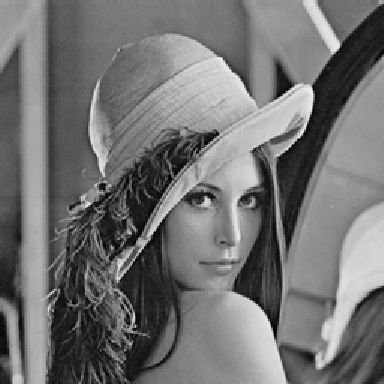
\includegraphics[clip, width=\textwidth]{figure/Lenna.pdf}
    \caption{入力画像}
    \label{fig:input_example}
  \end{minipage}
  \begin{minipage}{.45\hsize}
    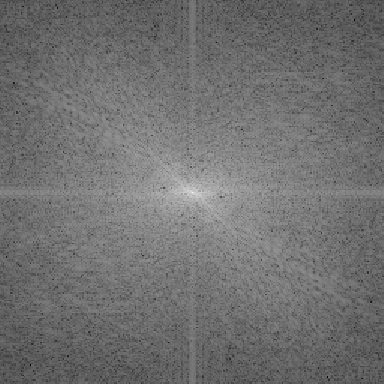
\includegraphics[clip, width=\textwidth]{figure/Lenna_dft.pdf}
    \caption{入力画像の周波数成分}
    \label{fig:dft_example}
  \end{minipage}
\end{figure}
\fi

\section{ハイパスフィルタによる画像処理}

\autoref{code:high_pass}に,画像に対してハイパスフィルタを行う$\mathsf{high\_pass\_img}()$関数を示す.
\autoref{code:high_pass}では,入力された画像から離散フーリエ変換を用いて周波数成分を抽出し,
$x, y$それぞれのカットオフ周波数より低い周波数領域に0を代入したのちに離散フーリエ逆変換
を用いて画像へと復元する.ただし,処理時間の都合上,離散フーリエ変換,逆変換はNumPy
ライブラリにて実装されている高速フーリエ変換を用いる.
\lstinputlisting[caption=画像へのハイパスフィルタを行う$\mathsf{high\_pass\_img}()$関数, label={code:high_pass}]{script/show_high_pass.py}

\autoref{fig:high_input}に入力画像,
\autoref{fig:high_pass_dft}に\autoref{fig:dft_high}に対してハイパスフィルタで
処理した後の周波数成分,
\autoref{fig:high_pass_idft}に復元した出力画像を示す.
\autoref{fig:high_pass_idft}より,画像内の顔の輪郭や髪の毛などといったよなピクセル間の
温度差の激しい部分,すなわちエッジが抽出できており,
逆に帽子の模様や鏡の縁のようなピクセル間の温度差が類似している部分が除去されている.
このことから,画像データに対してハイパスフィルタを用いることにより
画像のエッジ抽出として活用することができる.

\iffigure
\begin{figure}[h]
  \centering
  \begin{minipage}{.25\hsize}
    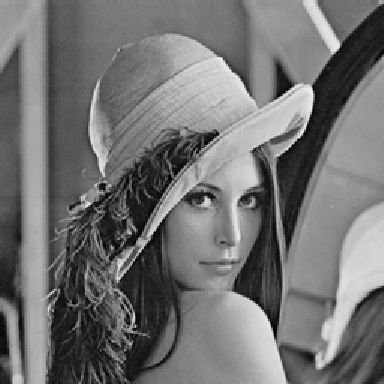
\includegraphics[clip, width=\textwidth]{figure/Lenna.pdf}
    \caption{入力画像}
    \label{fig:high_input}
  \end{minipage}
  \begin{minipage}{.25\hsize}
    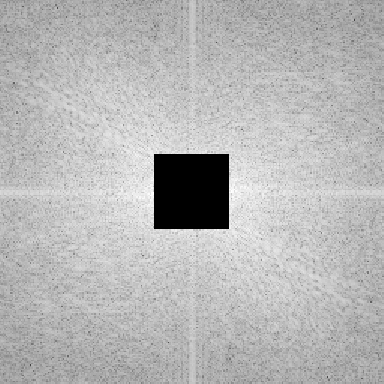
\includegraphics[clip, width=\textwidth]{figure/high_pass_dft_2d.pdf}
    \caption{ハイパスフィルタによる抽出}
    \label{fig:high_pass_dft}
  \end{minipage}
  \begin{minipage}{.25\hsize}
    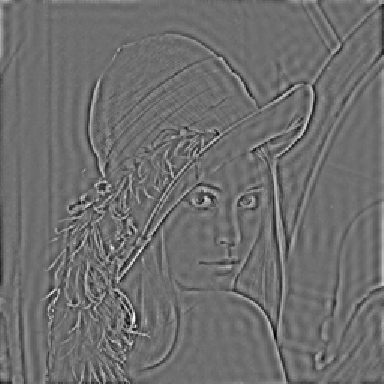
\includegraphics[clip, width=\textwidth]{figure/high_pass_idft_2d.pdf}
    \caption{処理後の画像}
    \label{fig:high_pass_idft}
  \end{minipage}
\end{figure}
\fi

\section{ローパスフィルタのによる画像処理}

\autoref{code:low_pass}に,画像に対してローパスフィルタを行う$\mathsf{low\_pass\_img}()$関数を示す.
\autoref{code:low_pass}では,\autoref{code:low_pass}と同様に
入力された画像の周波数成分を抽出し, $x, y$それぞれのカットオフ周波数より高い周波数領域
に0を代入したのちに逆変換を用いて画像へと復元する.
\lstinputlisting[caption=画像へのローパスフィルタを行う$\mathsf{low\_pass\_img}()$関数, label={code:low_pass}]{script/show_low_pass.py}

\autoref{fig:low_input}に入力画像,
\autoref{fig:low_pass_dft}に\autoref{fig:dft_low}に対してローパスフィルタで
処理した後の周波数成分,
\autoref{fig:low_pass_idft}に復元した出力画像を示す.
\autoref{fig:low_pass_idft}と\autoref{fig:low_input}を比較すると,
画像内の輪郭がぼやけており鮮明さが失われていることがわかる.
このことから,画像データに対してローパスフィルタを用いると画像に対してぼかしをかける
処理として活用することができる.

\iffigure
\begin{figure}[h]
  \centering
  \begin{minipage}{.25\hsize}
    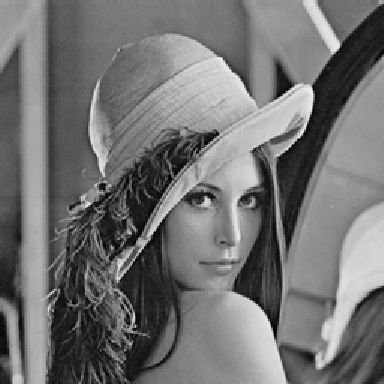
\includegraphics[clip, width=\textwidth]{figure/Lenna.pdf}
    \caption{入力画像}
    \label{fig:low_input}
  \end{minipage}
  \begin{minipage}{.25\hsize}
    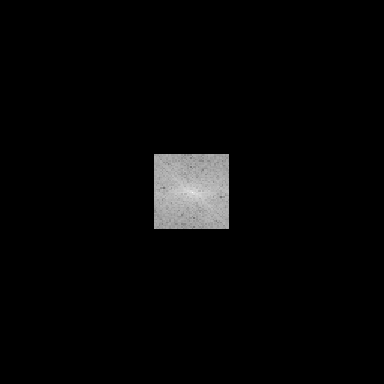
\includegraphics[clip, width=\textwidth]{figure/low_pass_dft_2d.pdf}
    \caption{ローパスフィルタによる抽出}
    \label{fig:low_pass_dft}
  \end{minipage}
  \begin{minipage}{.25\hsize}
    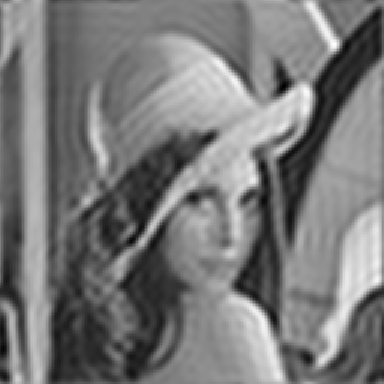
\includegraphics[clip, width=\textwidth]{figure/low_pass_idft_2d.pdf}
    \caption{処理後の画像}
    \label{fig:low_pass_idft}
  \end{minipage}
\end{figure}
\fi


\chapter{結論}

本レポートでは,信号処理技術に用いられている離散フーリエ変換,
フィルタ処理の一部を画像データに活用する実験を行った.
結果として,データの高周波成分を抽出するハイパスフィルタは画像処理においては
エッジ抽出として活用でき,データの低周波成分を抽出するローパスフィルタは
画像処理におけるぼかしをかける処理として活用できることがわかった.

\end{document}
